\documentclass[../main_proj5.tex]{subfiles}

\graphicspath{{\subfix{figures/}}}

\begin{document}

\onecolumngrid
\appendix
\section{Appendix A}\label{app:p5_AppendixA}

\subsection{Deriving the discretized Schr\"odinger equation}\label{app:p5_AppendixA_discretized schrodinger}

Using the scaled schrodinger equation of equation \eqref{eq:p5_scaled_schrodinger_p5}

\begin{equation}
    \label{eq:appA_scaled_schrodinger}
    \text{i}\frac{\partial u}{\partial t} =
    -\frac{\partial^{2}u}{\partial x^{2}} - \frac{\partial^{2} u}{\partial y^{2}} + v(x,y ) u \quad,
\end{equation}

\noindent we want to discretize using the Crank-Nicolson method. For this discretization the following notation and variables are introduced: 
\begin{itemize}
    \item Domains: $x\in[0, 1]$, $y\in[0, 1]$ $t\in[0, T]$
    \item Stepsize: $h$ for $x$ and $y$, $\Delta t$ for t
    \item Discretization: $x \rightarrow x_i = i h$, with $i = 0, 1, \ldots, M-1$, $y \rightarrow y_j = j h$, with $j = 0, 1, \ldots, M-1$ and $t \rightarrow t_n = n \Delta t$, with $n = 0, 1, \ldots, N_t-1$
    \begin{itemize}
        \item $u(x,y,t) \rightarrow u(ih,jh,n \Delta t) \equiv u_{ij}^n$
        \item $v(x,y) \rightarrow v(ih,jh) \equiv v_{ij}$
        \item $F(x, y, t)\rightarrow F(ih,jh,n \Delta t) \equiv F_{ij}^n$
        \item derivatives becomes $\frac{\partial u(x,y,t)}{\partial x} = \left(\frac{\partial u}{\partial x}\right)_{ij}^{n}$
    \end{itemize}
\end{itemize}

The general form of the original Crank-Nicolson scheme for an equation of the form $\frac{\partial u}{\partial t} = F(x, y, t)$ is 

\begin{equation}
    \label{eq:app_p5_general_Crank_Nicolson}
    \left(\frac{\partial u}{\partial t} \right)_{ij}^n = 
    \frac{1}{2}\left[F_{ij}^{n+1} + F_{ij}^{n}\right] \quad, 
\end{equation}

\noindent where we have introduced a similar short-hand notation for the derivatives and $F$ as that of $u$. For equation \eqref{eq:appA_scaled_schrodinger} this implies that 

\begin{equation*}
    F(x,y,t) = \frac{1}{\text{i}}\left(-\frac{\partial^{2}u}{\partial x^{2}} - \frac{\partial^{2} u}{\partial y^{2}} + v(x,y ) u\right) \quad.
\end{equation*}

\noindent Using the forward difference for the first-order partial derivatives and the general form for the second-order partial derivatives the discretized versions can be expressed as 

\begin{equation*}
    \left(\frac{\partial u}{\partial t} \right)_{ij}^n = \frac{u_{ij}^{n+1} -u_{ij}^{n}}{\Delta t} + \mathcal{O}(\Delta t)\quad, 
\end{equation*}
\begin{equation*}
    \left(\frac{\partial^{2} u}{\partial x^{2}} \right)_{ij}^{n(+1)} 
    = \frac{u_{i+1, j}^{n(+1)} -2u_{ij}^{n(+1)} + u_{i-1, j}^{n(+1)}}{h^{2}} 
    +\mathcal{O}(h^{2})\quad, \text{ and}
\end{equation*}
\begin{equation*}
    \left(\frac{\partial^{2} u}{\partial y^{2}} \right)_{ij}^{n(+1)} 
    = \frac{u_{i, j+1}^{n(+1)} -2u_{ij}^{n(+1)} + u_{i, j-1}^{n(+1)}}{h^{2}} 
    +\mathcal{O}(h^{2})\quad.
\end{equation*}

\noindent Here we use the superscript $n(+1)$ to denote the derivatives associated with $F_{ij}^n$ and $F_{ij}^{n+1}$ by ignoring/including the content of the parentheses, respectively. By using the approximate terms for the derivatives (i.e. omitting the terms; $\mathcal{O}(\Delta t)$ and $\mathcal{O}(h^{2})$) and substituting into equation \eqref{eq:app_p5_general_Crank_Nicolson} we get

\begin{equation}
\begin{split}
    \text{i}\left(\frac{\partial u}{\partial t} \right)_{ij}^n 
    & = \frac{1}{2}\left(
    -\left(\frac{\partial^{2}u}{\partial x^{2}}\right)_{ij}^{n+1} 
    - \left(\frac{\partial^{2} u}{\partial y^{2}}\right)_{ij}^{n+1} 
    + v_{ij} u_{ij}^{n+1}
    \right)
    + \frac{1}{2}\left( 
    -\left(\frac{\partial^{2}u}{\partial x^{2}}\right)_{ij}^{n} 
    - \left(\frac{\partial^{2} u}{\partial y^{2}}\right)_{ij}^{n} 
    + v_{ij} u_{ij}^{n}
    \right) \\
    \text{i} \frac{u_{i,j}^{n+1} - u_{i,j}^{n}}{\Delta t} &=
    \frac{1}{2}\left(
    - \frac{u_{i+1, j}^{n+1} -2u_{ij}^{n+1} + u_{i-1, j}^{n+1}}{h^{2}} 
    - \frac{u_{i, j+1}^{n+1} -2u_{ij}^{n+1} + u_{i, j-1}^{n+1}}{h^{2}} 
    + v_{ij} u_{ij}^{n+1}
    \right) \\
    &+\frac{1}{2}\left(
    - \frac{u_{i+1, j}^{n} -2u_{ij}^{n} + u_{i-1, j}^{n}}{h^{2}} 
    - \frac{u_{i, j+1}^{n} -2u_{ij}^{n} + u_{i, j-1}^{n}}{h^{2}} 
    + v_{ij} u_{ij}^{n}
    \right) \quad.
    \end{split}   
\end{equation}

\noindent Next we: 
\begin{enumerate}
    \item Sort all $n+1$ terms to the left hand side and all $n$ terms to the right hand side
    
\begin{equation*} 
\begin{split} 
\text{i} \frac{u_{i,j}^{n+1}}{\Delta t} &- \frac{1}{2}\left( -\frac{u_{i+1, j}^{n+1} -2u_{ij}^{n+1} + u_{i-1, j}^{n+1}}{h^{2}} - \frac{u_{i, j+1}^{n+1} -2u_{ij}^{n+1} + u_{i, j-1}^{n+1}}{h^{2}} + v_{ij} u_{ij}^{n+1} \right) = \\& 
\text{i} \frac{u_{i,j}^{n}}{\Delta t} + \frac{1}{2}\left(-\frac{u_{i+1, j}^{n} -2u_{ij}^{n}  u_{i-1, j}^{n}}{h^{2}} - \frac{u_{i, j+1}^{n} -2u_{ij}^{n} + u_{i, j-1}^{n}}{h^{2}} + v_{ij} u_{ij}^{n} \right) 
\end{split}
\end{equation*}

    \item Pull $-1/h^{2}$ out from the parenthesizes.

\begin{equation*} 
\begin{split} 
\text{i} \frac{u_{i,j}^{n+1}}{\Delta t} &+ \frac{1}{2h^{2}}\left( u_{i+1, j}^{n+1} -2u_{ij}^{n+1} + u_{i-1, j}^{n+1} + u_{i, j+1}^{n+1} -2u_{ij}^{n+1} + u_{i, j-1}^{n+1} - h^{2} v_{ij} u_{ij}^{n+1} \right) = \\& 
\text{i} \frac{u_{i,j}^{n}}{\Delta t} - \frac{1}{2h^{2}}\left(u_{i+1, j}^{n} -2u_{ij}^{n} + u_{i-1, j}^{n} + u_{i, j+1}^{n} -2u_{ij}^{n} + u_{i, j-1}^{n} - h^{2} v_{ij} u_{ij}^{n} \right) 
\end{split}
\end{equation*}

    \item Multiply through the equation with $\text{i}/\text{i}$, use $\text{i}^{2}=-1$ and multiply through the equation with $-\text{i}\Delta t$.
    
\begin{equation*} 
\begin{split} 
u_{i,j}^{n+1} &- \frac{\text{i}\Delta t}{2h^{2}}\left( u_{i+1, j}^{n+1} -2u_{ij}^{n+1} + u_{i-1, j}^{n+1} + u_{i, j+1}^{n+1} -2u_{ij}^{n+1} + u_{i, j-1}^{n+1} - h^{2} v_{ij} u_{ij}^{n+1} \right) = \\& 
 u_{i,j}^{n} + \frac{\text{i}\Delta t}{2h^{2}}\left(u_{i+1, j}^{n} -2u_{ij}^{n} + u_{i-1, j}^{n} + u_{i, j+1}^{n} -2u_{ij}^{n} + u_{i, j-1}^{n} - h^{2} v_{ij} u_{ij}^{n} \right) 
\end{split}
\end{equation*}

    \item Define $r:=\text{i}\Delta t/2h^{2}$ and split the parenthesis into one for each part of $F(x,y,t)$.

\begin{equation}
\begin{split} 
u_{i,j}^{n+1} &- r\left( u_{i+1, j}^{n+1} -2u_{ij}^{n+1} + u_{i-1, j}^{n+1}\right) -r \left(u_{i, j+1}^{n+1} -2u_{ij}^{n+1} + u_{i, j-1}^{n+1}\right) + \frac{\text{i}\Delta t}{2} v_{ij} u_{ij}^{n+1}= \\& 
 u_{i,j}^{n} + r\left(u_{i+1, j}^{n} -2u_{ij}^{n} + u_{i-1, j}^{n}\right) + r \left(u_{i, j+1}^{n} -2u_{ij}^{n} + u_{i, j-1}^{n}\right) - \frac{\text{i}\Delta t}{2} v_{ij} u_{ij}^{n} 
\quad. 
\end{split}
\end{equation}
\end{enumerate}   

This is the Crank-Nicolson discretized scaled schrodinger equation in the two-dimensional position space. 

\newpage

\subsection{Deriving the matrix-vector equation for the discretized Schr\"odinger equation}\label{app:p5_AppendixA_matrix_vector}


Using equation \eqref{eq:p5_discretized_schrodinger_crank_nicolson} we see that the Crank-Nicolson scheme in two spatial dimensions and the temporal dimension will involve in total 5 spatial points from each time step. The computational stencil for the propagation forward in time, to $t=n+1$ for $t=n$, is illustrated in Figure \ref{fig:p5_comp_stencil_CNCS}. 

\begin{figure}[h!]
    \centering
    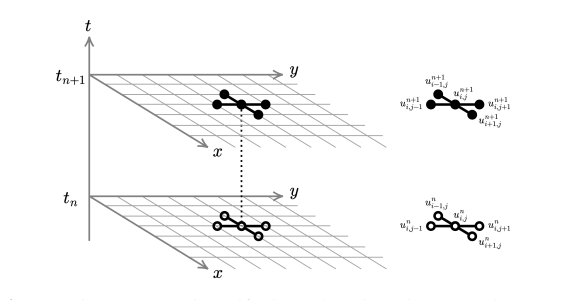
\includegraphics[width=0.6\linewidth]{Project 5/figures/comp_stencil_CNCS.png}
    \caption{The computational stencil for the Crank-Nicolson scheme in two spatial dimensions + the temporal. The propagation forward in time to $t=n+1$ implies using the four closest spatial neighbors in $t=n$. Figure from lecture notes in FYS3150 UiO \cite{lecture_notes}.}
    \label{fig:p5_comp_stencil_CNCS}
\end{figure}

\noindent To solve equation \eqref{eq:p5_discretized_schrodinger_crank_nicolson} for the whole discretzed space it is benefitial to express it in terms of a matrix-vector equation on the form 

\begin{equation}
    A \mathbf{u}^{n+1} = B    \mathbf{u}^{n} .
\end{equation}

\noindent To derive the structure of the components of this equation, we will consider a discretization of the x,y-plane with $M=5$. This implies that we will have $N_{int}=3$ internal points in each plane yielding $N_{int}^{2}=9$ internal points in total. Figure \ref{fig:p5_M5_discretized_xyplane} shows what the x,y plane look like for this discretization.

\begin{figure}[h!]
    \centering
    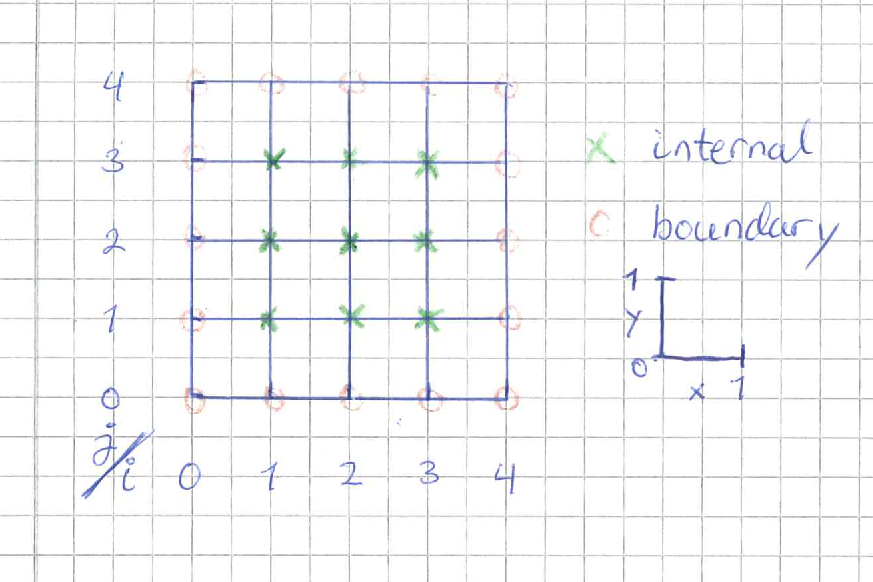
\includegraphics[width=0.6\linewidth]{Project 5/figures/discrtetization_xy.png}
    \caption{The x,y plane discretized using $M=5$ points in each dimension. Here we see how the $i$ index belongs to the x-plane and $j$ to y. }
    \label{fig:p5_M5_discretized_xyplane}
\end{figure}

\noindent Some important definitions for the discretization:

\begin{itemize}
    \item To keep track of the value of the scaled schrodinger equation at time $n$ we let $U^{n(+1)} \in \mathbb{C}^{M\times M}$ be the matrix that hold all the values $u_{i,j}^{n(+1)}$.
    \item Similarly, we use the matrix $V \in \mathbb{R}^{M \times M}$ to hold all the values for the external potential $v_{ij}$.
    \item To confine the total probability given by Born's rule to this space we use Drichlet boundary conditions, that is, $u(x,y,t) = 0,$ for all instances where $x || y = 0$.
    \item Next we let the $j$ and $i$ index of the y- and x-coordinate signify the rows and columns of our matrices. 
\end{itemize}   

\noindent As a result of these choices we know that every boundary point is $0$ so we do not need to solve \eqref{eq:p5_discretized_schrodinger_crank_nicolson} for these. Considering only the left-hand-side of \eqref{eq:p5_discretized_schrodinger_crank_nicolson} we can rewrite it as

\begin{equation*}
    u_{i,j}^{n+1}(1 + 4r + \text{i} \frac{\Delta t}{2} v_{i,j}) 
    - r(u_{i,j+1}^{n+1} +u_{i,j-1}^{n+1} + u_{i+1,j}^{n+1} u_{i-1,j}^{n+1}) .
\end{equation*}

\noindent If we write this equation out for every combination of $i,j$ in the internal points this yields;
$$
\begin{array}{ccc|ccc|ccc|ccc}
&     & j       &    & 1 &                    &    & 2 &                     &   & 3 &                       \\
&     & i       &  1 & 2 & 3                  &  1 & 2 & 3                   & 1 & 2 & 3                    \\
j & i &         & u_{1,1}^{n+1} & u_{2,1}^{n+1} & u_{3,1}^{n+1} &  u_{1,2}^{n+1} & u_{2,2}^{n+1} & u_{3,2}^{n+1} & u_{1,3}^{n+1} & u_{2,3}^{n+1} & u_{3,3}^{n+1}  \\ \hline
  & 1 & u_{1,1}^{n+1} &  a_{0} & -r & 0 & -r & 0 & 0  & 0 & 0 & 0 \\
1 & 2 & u_{2,1}^{n+1} &  -r & a_{1} & -r &  0 & -r & 0 & 0 & 0 & 0  \\
  & 3 & u_{3,1}^{n+1} &  0 & -r & a_2 &  0 & 0 & -r &  0 & 0 & 0  \\ \hline
& & \vdots & &  \vdots &&& \vdots &&&  \vdots &  \\ \hline
&   1 & u_{1,3}^{n+1} & 0 & 0 & 0 & -r & 0 & 0 &  a_{6} & -r & 0  \\
3 & 2 & u_{2,3}^{n+1} & 0 & 0 & 0 & 0 & -r & 0 &  -r & a_7 & -r \\
&   3 & u_{3,3}^{n+1} & 0 & 0 & 0 & 0 & 0 & -r &  0 & -r & a_8  \\ 
\end{array} 
$$

\noindent where we have introduced $a_k = 1 + 4r + \text{i} \frac{\Delta t}{2} v_{ij}$ with $k=(i-1)N_{int} + j - 1$. We let this be the matrix $A$ and let $\mathbf{u}^{n+1}$ be (on row form) $\mathbf{u^{n+1}} = [u_{1,1}^{n+1}, u_{2,1}^{n+1}, ..., u_{2,3}^{n+1}, u_{3,3}^{n+1}]$. In the same way we can write the right hand side of equation \eqref{eq:p5_discretized_schrodinger_crank_nicolson} as 

\begin{equation*}
    u_{i,j}^{n+1}(1 - 4r - \text{i} \frac{\Delta t}{2} v_{i,j}) 
    + r(u_{i,j+1}^{n+1} +u_{i,j-1}^{n+1} + u_{i+1,j}^{n+1} u_{i-1,j}^{n+1}) .
\end{equation*}

\noindent which written for every $i,j$ pair yields the same structure as $A$ only with $b_k = 1 -4r - \text{i} \frac{\Delta t}{2} v_{i,j}$ and with $r$ instead of $-r$ on the diagonals. 

\newpage
\subsection{Extra figures}\label{app:p5_AppendixA_Extra_figures}

Extra figures showing the time evolution for the real and imaginary part of the wave functionat  t= 0.0, 0.001 and 0.002.

\begin{figure}[h!]
    \centering
    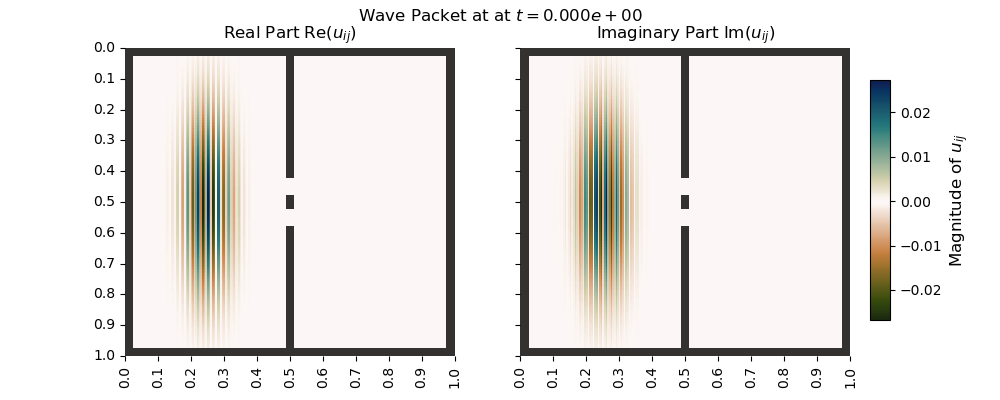
\includegraphics[width=0.75\linewidth]{Project 5/figures/problem8and9_M201_Nslits2_uij_000.png}
    \caption{The real (left panel) and imaginary (right panel) part of the scale wave function at $t=0.0$, That is $U^{0}$. Note the color bars have different scales for each figure.}
    \label{fig:enter-label}
\end{figure}

\begin{figure}[h!]
    \centering
    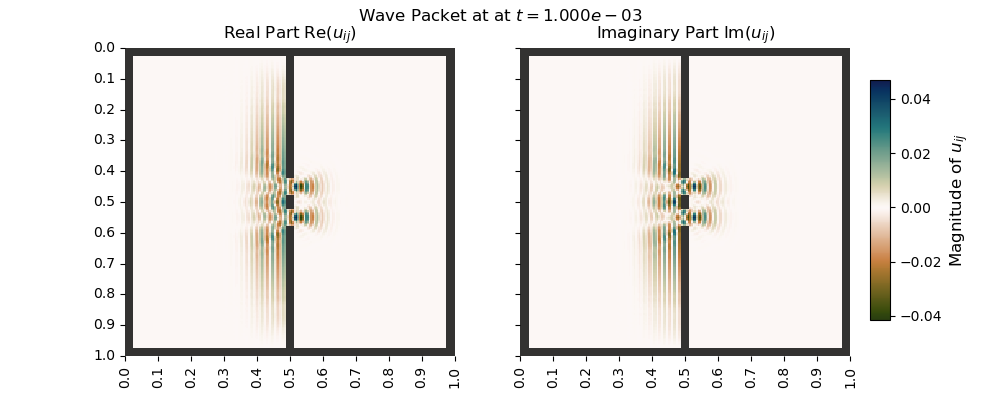
\includegraphics[width=0.75\linewidth]{Project 5/figures/problem8and9_M201_Nslits2_uij_040.png}
    \caption{The real (left panel) and imaginary (right panel) part of the scale wave function at $t=0.0$, That is $U^{40}$ when using $\Delta t = 2.5*1e-5$. Note the color bars have different scales for each figure.}
    \label{fig:enter-label}
\end{figure}

\begin{figure}[h!]
    \centering
    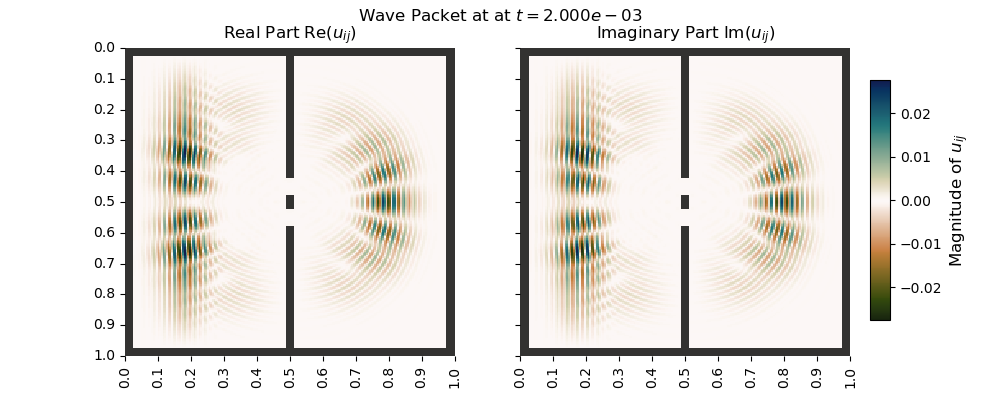
\includegraphics[width=0.75\linewidth]{Project 5/figures/problem8and9_M201_Nslits2_uij_080.png}
    \caption{The real (left panel) and imaginary (right panel) part of the scale wave function at $t=0.0$, That is $U^{80}$ when using $\Delta t = 2.5*1e-5$. Note the color bars have different scales for each figure.}
    \label{fig:fig3a}
\end{figure}

\newpage

\begin{figure}
    \centering
    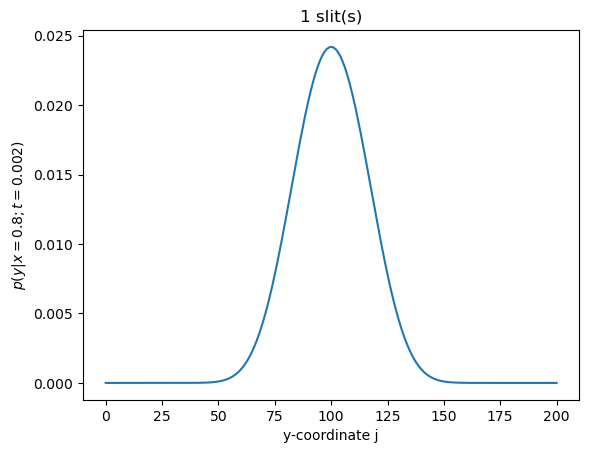
\includegraphics[width=0.5\linewidth]{Project 5/figures/marg_distribution_x08_t0002_Nslits1.png}
    \caption{The marginal distribution for a single slit experiment at $x=0.8$ and $t=0.002$.}
    \label{fig:marg_1slits}
\end{figure}
\begin{figure}
    \centering
    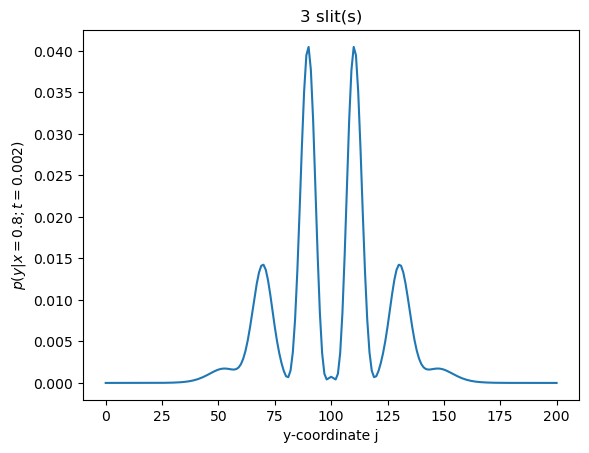
\includegraphics[width=0.5\linewidth]{Project 5/figures/marg_distribution_x08_t0002_Nslits3.png}
    \caption{The marginal distribution for a triple slit experiment at $x=0.8$ and $t=0.002$.}
    \label{fig:marg_3slits}
\end{figure}
\end{document}


